\documentclass{beamer}
%\usepackage{enumitem}
\usepackage{graphicx}
\usepackage[english]{babel}
\usepackage[latin1]{inputenc}
\usepackage{times}
\usepackage[T1]{fontenc} 
% Or whatever. Note that the encoding and the font should match. If T1
% does not look nice, try deleting the line with the fontenc.
\usepackage{amsmath}
\usepackage{color}
\usepackage{rotating}
\usepackage{tabu}
\usepackage{pgfpages}

\mode<presentation>
{
	%\usetheme{Madrid}
	\usetheme{CambridgeUS}
	%\usecolortheme{seahorse}
	\setbeamercovered{transparent}
	\beamertemplatenavigationsymbolsempty
	% \setbeameroption{show notes}
	% \setbeameroption{show notes on second screen}
}

\newcommand{\linespace}{\vskip 0.25cm}

\definecolor{MyForestGreen}{rgb}{0,0.7,0} 
\newcommand{\tableemph}[1]{{#1}}
\newcommand{\tablewin}[1]{\tableemph{#1}}
\newcommand{\tablemid}[1]{\tableemph{#1}}
\newcommand{\tablelose}[1]{\tableemph{#1}}

\definecolor{MyLightGray}{rgb}{0.6,0.6,0.6}
\newcommand{\tabletie}[1]{\color{MyLightGray} {#1}}

% The text in square brackets is the short version of your title and will be used in the
% header/footer depending on your theme.
\title[Improving generalization via simplification]{Improving Generalization of Evolved Programs through Automatic Simplification}

% Sub-titles are optional - uncomment and edit the next line if you want one.
% \subtitle{Why does sub-tree crossover work?} 

% The text in square brackets is the short version of your name(s) and will be used in the
% header/footer depending on your theme.
\author[Helmuth, McPhee, et al]{Thomas Helmuth, Nic McPhee\inst{1}, Edward Pantridge, \& Lee Spector}

% The text in square brackets is the short version of your institution and will be used in the
% header/footer depending on your theme.
\institute[]
{
	\inst{1} Division of Science and Mathematics \\
	University of Minnesota, Morris \\
	Morris, Minnesota, USA
}

% The text in square brackets is the short version of the date if you need that.
\date[GECCO 2017]{18 July -- GECCO 2017 -- Berlin}

% Delete this, if you do not want the table of contents to pop up at
% the beginning of each subsection:
\AtBeginSection[]
{
  \begin{frame}<beamer>
    \frametitle{Outline}
    \tableofcontents[currentsection, hideothersubsections]
  \end{frame}
}

\begin{document}

\begin{frame}
  \titlepage
\end{frame}

\section*{The Big Picture}

\subsection*{Simplify your life}

\begin{frame}{Simplification: Can be good in multiple ways}
		
\begin{columns}
% Column 1
\begin{column}{0.6\textwidth}
\begin{overprint}
	\onslide<1-2>
	\vspace{-1cm}
\begin{itemize}
	\item Simplifying programs is ``easy'' in Push~\cite{Spector:2014:GECCOcomp}
	\item Can dramatically shrink programs without changing their functionality
	\begin{itemize}
		\item Usually less than 50\% of original size, sometimes less than 5\%!
	\end{itemize}
	\item Simplification allows us to better understand evolved programs
	\item So far not great as a genetic operator 
\end{itemize}

\begin{center}
	 \textbf{but\ldots}
\end{center}

\onslide<3>

\vspace{-1cm}
\begin{center}
	\textbf{Can substantially improve generalization!}
\end{center}

\begin{itemize}
	\item Using multiple simplification methods
	\item Tested across dozens of software synthesis problems
\end{itemize}

~

\begin{itemize}
	\item 65\% of programs generalized before simplification 
	\item 76\% generalized after simplification
	\item Size correlates with generalization
\end{itemize}

\end{overprint}

\end{column}
% Column 2
\begin{column}{0.4\textwidth}
	\begin{overprint}
		\onslide<1>
		\begin{center}
		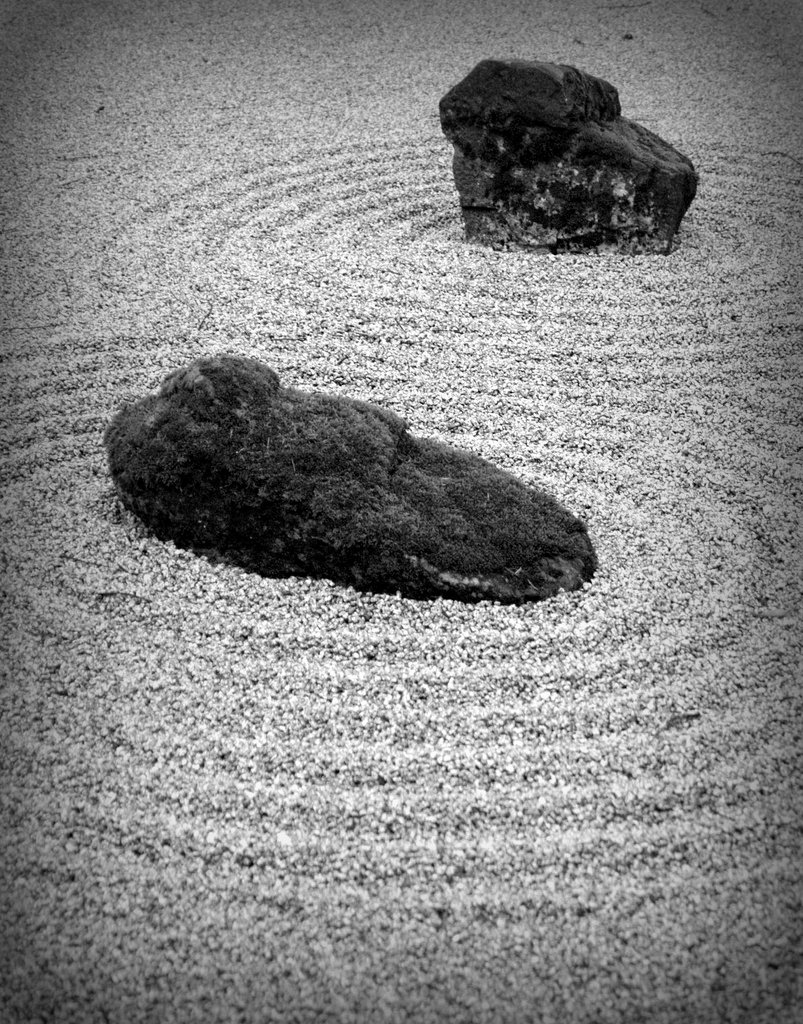
\includegraphics[height=0.7\textheight]{Illustrations/zen.jpg} \\
		\tiny \url{https://www.flickr.com/photos/lauradeponte/2236562103/}
		\end{center} 
		\onslide<2>
		\begin{center}
		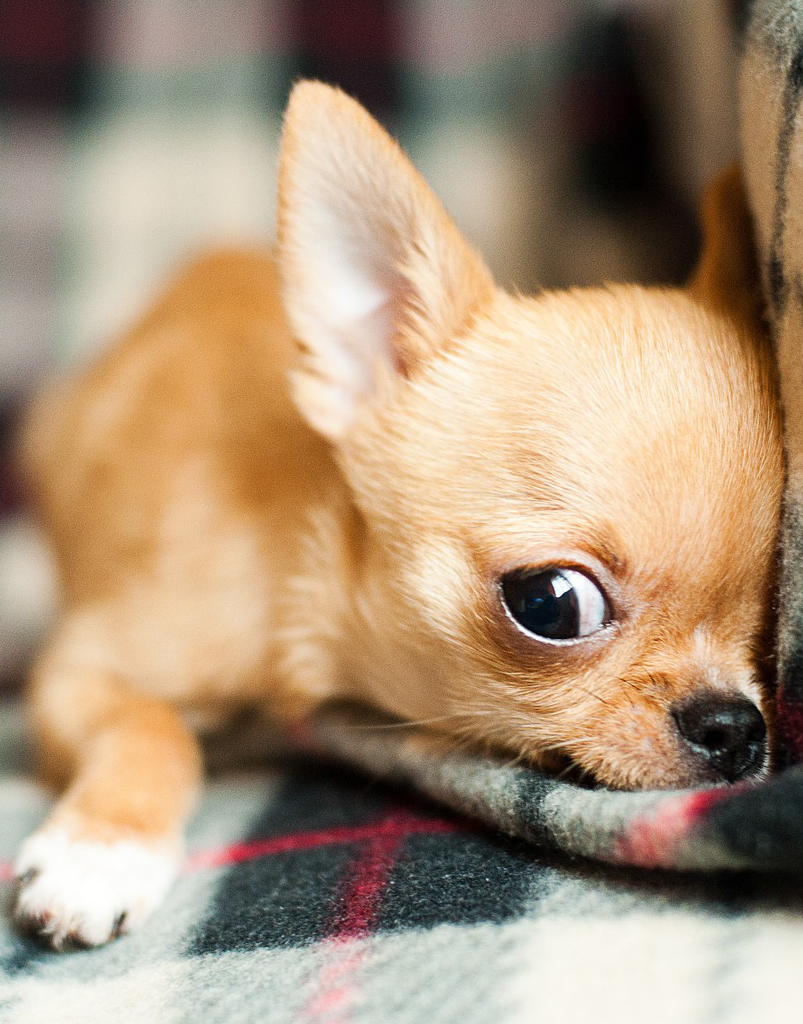
\includegraphics[height=0.7\textheight]{Illustrations/chihuahua-smaller} \\
		\tiny \url{https://pixabay.com/p-820086/}
		\end{center} 
		\onslide<3>
		\begin{center}
		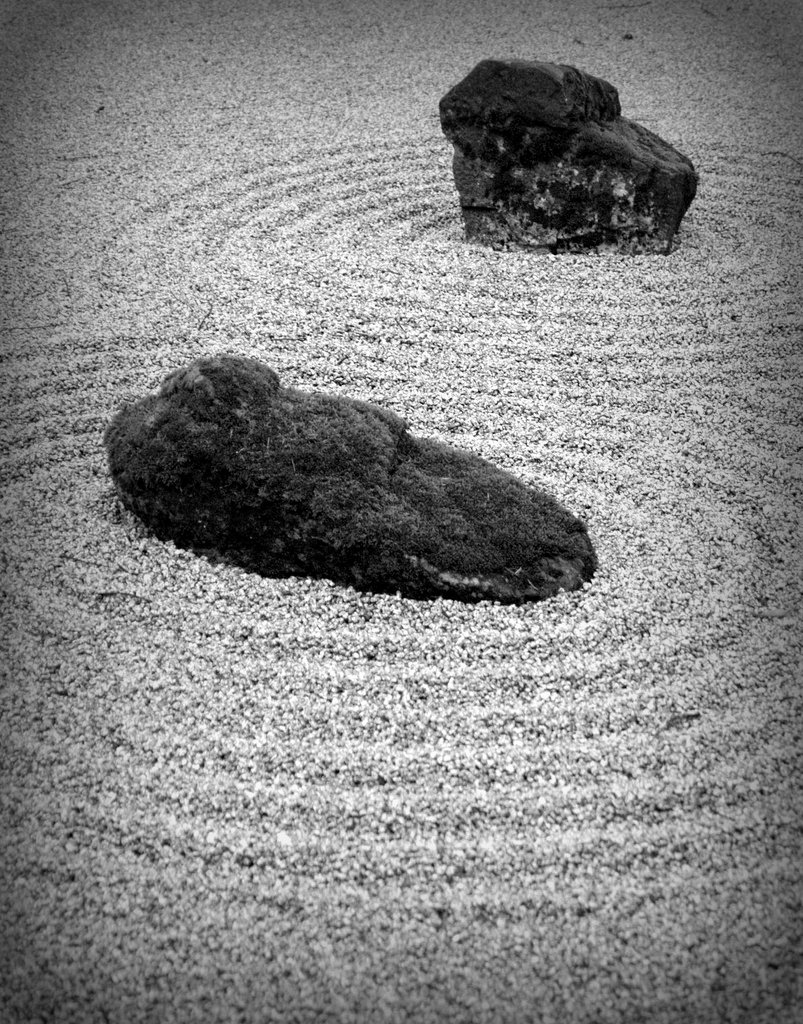
\includegraphics[height=0.7\textheight]{Illustrations/zen.jpg} \\
		\tiny \url{https://www.flickr.com/photos/lauradeponte/2236562103/}
		\end{center} 
	\end{overprint}
\end{column}
\end{columns}

\note{Remember to switch to the cute dog!}

\end{frame}

\subsection*{Outline}

\begin{frame}{Outline}
  \tableofcontents[hideallsubsections]
\end{frame}

%~~~~~~~~~~Background~~~~~~~~~~~~~~~~~~~~~~~~~~~~~~~~~~~~~~~~~~~~~~~~~~~~~~~~~~~~~~~~~~~~~~~~~~~~~~~~~~~~~~~

\section{Background}

\subsection{Push \& Plush}

\begin{frame}{Push: Stack-based GP}
In PushGP:
\begin{itemize}
	\item Instructions read data from and write to typed stacks
	\item E.g., \texttt{string-length} reads a value from the \texttt{string} stack, and writes the length of that string to the \texttt{integer} stack
	\item Programs are nested sequences of instructions
	\item Forgiving; data flows through stacks instead of syntax
\end{itemize}
Every Push program ``works''!

~

Clojush, a Clojure implmentation of PushGP, uses \emph{Plush genomes}~\cite{Helmuth:2016:GPTP}:
\begin{itemize}
	\item A linear sequence of \emph{genes}
	\item Each gene contains an instruction along with other metadata
	\begin{itemize}
		\item Includes a \emph{silent} flag that can be used to disable a gene
	\end{itemize}
\end{itemize}

~

Every Plush genome generates a working Push program!

\end{frame}

\subsection{Early simplification}

\begin{frame}{Ad hoc simplification}
Because \emph{every} Push program is ``legal'' and will execute, it's easy to (try to) simplify evolved structures through simple hill-climbing~\cite{Spector:2014:GECCOcomp}:
\begin{itemize}
	\item Remove some random stuff (e.g., an instruction)
	\item See if that changed things (by re-running the tests)
	\item Put the instruction(s) back if removal changed things; otherwise keep simplifying from there
\end{itemize}
 
 ~
 
 Substantially shortens end-of-run evolved programs and makes it much easier to
 understand them.
 \begin{itemize}
 	\item E.g., simplified 194 instructions down to just 9
 \end{itemize}
\end{frame}

\subsection{Surprising generalization}

\begin{frame}{``Accidental'' improvements in generalization}

Each problem has a set of \emph{training cases} and a set of \emph{test cases} for \emph{validation}~\cite{Helmuth:2015:GECCO}
\begin{itemize}
	\item Training cases are used during evolution to determine the quality of potential solutions
	\item Test cases are run after a solution has been found to gauge how well that program generalizes to unseen data
	\item We say a solution \emph{generalizes} if it has zero error on the unseen test cases
\end{itemize}

~

In~\cite{Helmuth:2015:dissertation} it was noted that this simplification (done primarily to improve readability) occasionally improved generalization:
\begin{itemize}
	\item Evolved solutions failed some unseen test cases
	\item Simplified versions, however, passed all the test cases
\end{itemize}

\note{Tom's dissertation notes that simplification improves generalization.}

\end{frame}

\subsection{(Lots of) related work}

\begin{frame}{Occam's razor? Or maybe not\ldots}
A long history of speculation and experimentation on the relationship between simplification and generalization in GP
\begin{itemize}
	\item Koza's first book~\cite{koza1992genetic} contains methods for simplifying programs
	\item Early focus often on simplification to make evolved programs easier to understand, and/or as a mechanism for bloat control
\end{itemize}

~

Also arguments that simpler programs are more likely to generalize~\cite{hooper:1996:iarGPes}
\begin{itemize}
	\item Short programs less likely (or capable) of ``memorizing'' noise
	\item E.g., include Minimum Description Length in the fitness~\cite{iba1994genetic}
\end{itemize}

~

\emph{However}
\begin{itemize}
	\item (Over)simplifying \emph{during} runs often appears harmful
	\item Possible that some large programs can act as \emph{ensembles} and generalize more effectively~\cite{gonccalves2015generalization}
\end{itemize}

\note{
	\begin{itemize}
		\item Do we want citations for the bloat stuff?
		\item There are citations for the simplifying during runs comment -- do we care?
	\end{itemize}
}

\end{frame}

\section{Exploring simplification}

\subsection{Experimental design}

\begin{frame}{The Big Plan}
Explore the impact of different \emph{post-run} simplification techniques on generalization in PushGP 

~

\begin{itemize}
	\item Five different simplification methods
	\item 24 software synthesis benchmark problems
\end{itemize}

~ 

Simplify 100 times for every evolved solution for each problem
\begin{itemize}
	\item How much do they simplify the programs?
	\item How many generalize?
\end{itemize} 

\end{frame}

\subsection{Simplification methods}

\begin{frame}{Simplification framework}

For each problem we have a set of
\begin{itemize}
	\item Training cases (usually hundreds)
	\item Test (or validation) cases (usually thousands)
\end{itemize}

~

Simplification is a simple hill climber trying to reduce size

~

Repeatedly (for a fixed number of steps):
\begin{itemize}
	\item Apply the simplification operator (more shortly)
	\item See if result generates the same errors on all the \emph{training} cases
	\item If it does, make it the current program; otherwise discard it
\end{itemize}

\note{
	\begin{itemize}
		\item 10K simplification steps
		\item Or 10 generations of GP with a pop size of 1K
		\item More than necessary in most cases, but we're only advocating doing this once at the end of runs, so not a huge expense
	\end{itemize}
}

~

Apply final result to the \emph{test} cases to see if it generalizes

\end{frame}

\begin{frame}{Five different simplification methods (First one)}

First method (\textbf{Program}) simplifies \emph{programs}
\begin{itemize}
	\item Original Push simplification method~\cite{Spector:2014:GECCOcomp}; pre-dates Plush
	\item Removes random program elements
	\begin{itemize}
		\item Instructions
		\item Blocks of code
		\item Pairs of parentheses
	\end{itemize}
\end{itemize}

\note{Removing a pair of parens flattens that section of the program}

\end{frame}

\begin{frame}{Five different simplification methods (Other four)}

Other four methods simplify Plush genomes, then convert to programs

~

Based on two primary operations
\begin{itemize}
	\item Silencing (and unsilencing) genes
%	\begin{itemize}
%		\item Ability to silence \& unsilence allows for backtracking
%	\end{itemize}
	\item Replacing instructions with NOOPs
%	\begin{itemize}
%		\item Can't be easily undone
%	\end{itemize}
\end{itemize}

\begin{center}
\begin{tabular}{r|cc} % {p{0.3\linewidth}cmp{0.3\linewidth}}
	&  Silencing & Silencing \& unsilencing \\ 
	\hline
	No NOOPs & \textbf{Genome} & \textbf{Genome-Backtracking} \\ 
	NOOPs & \textbf{Genome-Noop} & \textbf{Genome-Back\-tracking-Noop } \\ 
\end{tabular} 
\end{center}

\note{Say a little more about backtracking if there's time}

~

Additional details in the paper

\end{frame}

\subsection{Benchmark problems}

\begin{frame}{Benchmark problems}

24 software synthesis benchmark problems
\begin{itemize}
	\item Large subset of benchmark suite~\cite{Helmuth:2015:GECCO}
	\begin{itemize}
		\item The 24 of the 29 that we have solutions for
	\end{itemize}
	\item Some easy to solve, others much harder
	\item Solutions to some have high degree of generalization ``out of the box'', others have no solutions that generalize
\end{itemize}

\note{
	\begin{itemize}
		\item Taken from intro programming texts	
		\item 29 in suite
		\item 23 had generalizing solutions (if we count Checksum)
		\item Super Anagrams had 14 solutions, none of which generalized, but we included it just in case new simplification methods might fix that
		\item Every solution we had; nearly 800 solutions
	\end{itemize}
}

\end{frame}

\begin{frame}{Benchmark problems}
\begin{center}
	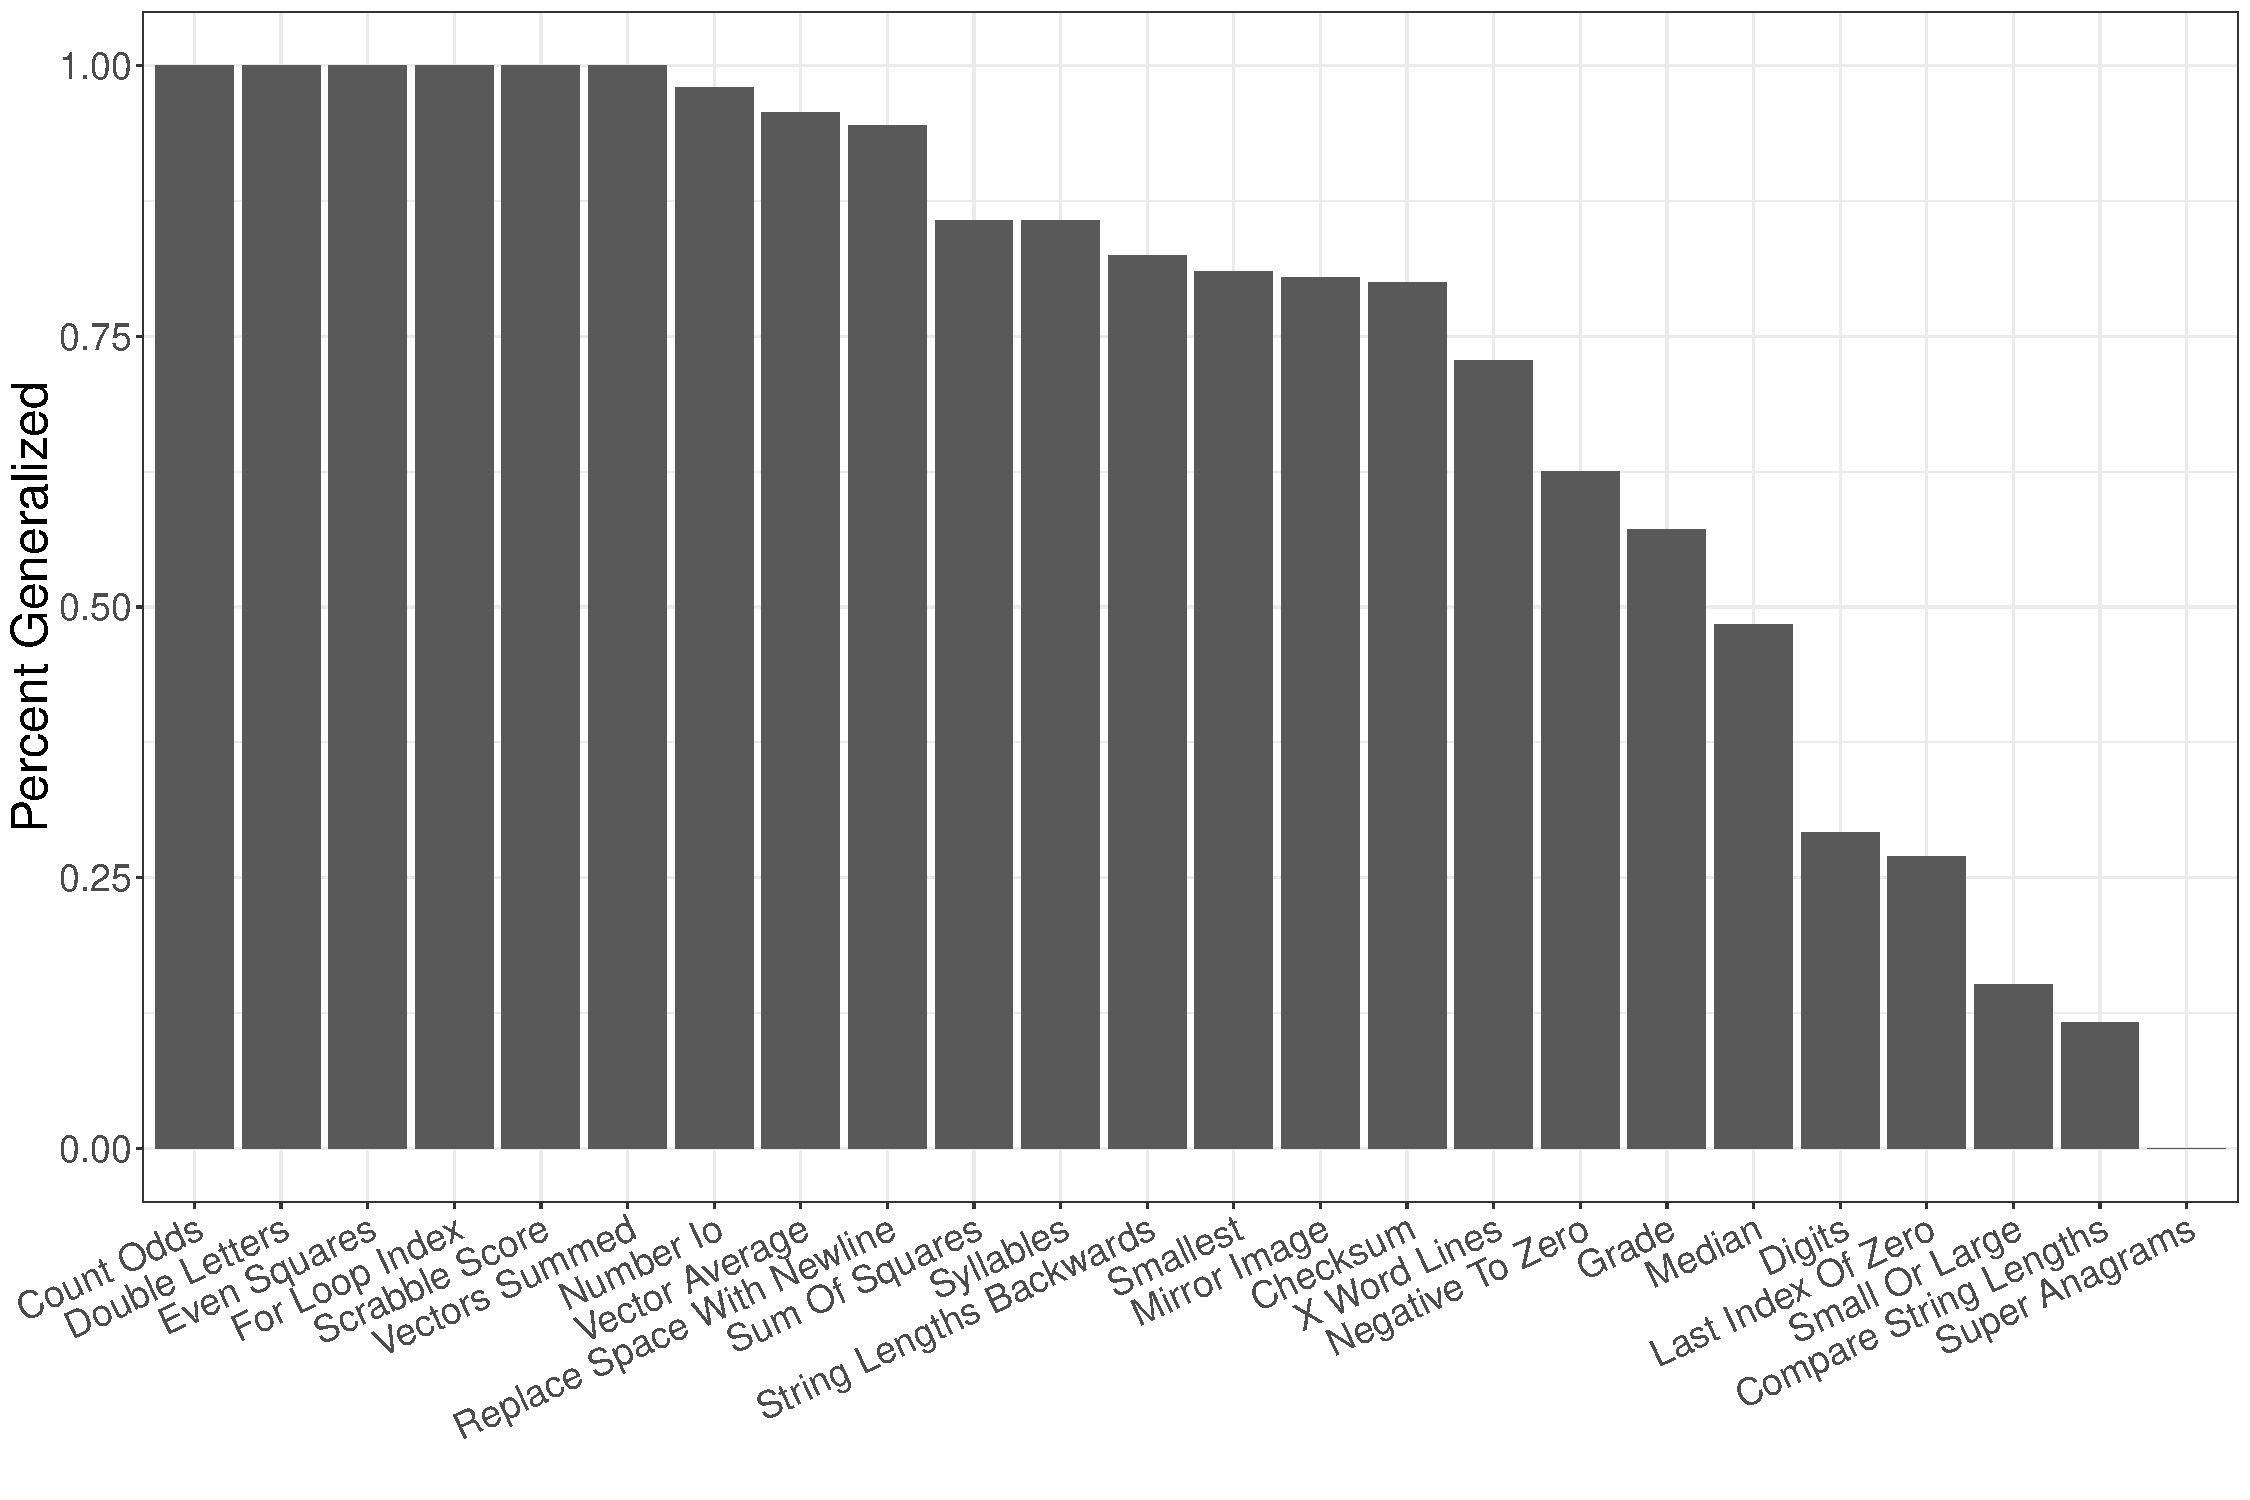
\includegraphics[width=0.95\linewidth]{Illustrations/Pct_gener_SLIDE}
\end{center}

\note{
	\begin{itemize}
		\item Count Odds has 8 solutions, all generalize
		\item Number IO has 100 solutions, almost all of which generalize
		\item Mirror Image has 97 solutions, about 80\% generalize
		\item Checksum has 5 solutions, 4 of which generalize
		\item Last Index Of Zero has 78 solutions, around a quarter generalize
		\item Super Anagrams has 14 solutions, none generalize
	\end{itemize}

Super anagrams might have trouble because it has binary outputs (so limited slope) [this is common to last three on slide 15].
}

\end{frame}

\section{Simplification results}

\subsection{Size reductions}

\begin{frame}{Substantial size reductions across the board}
\begin{center}
	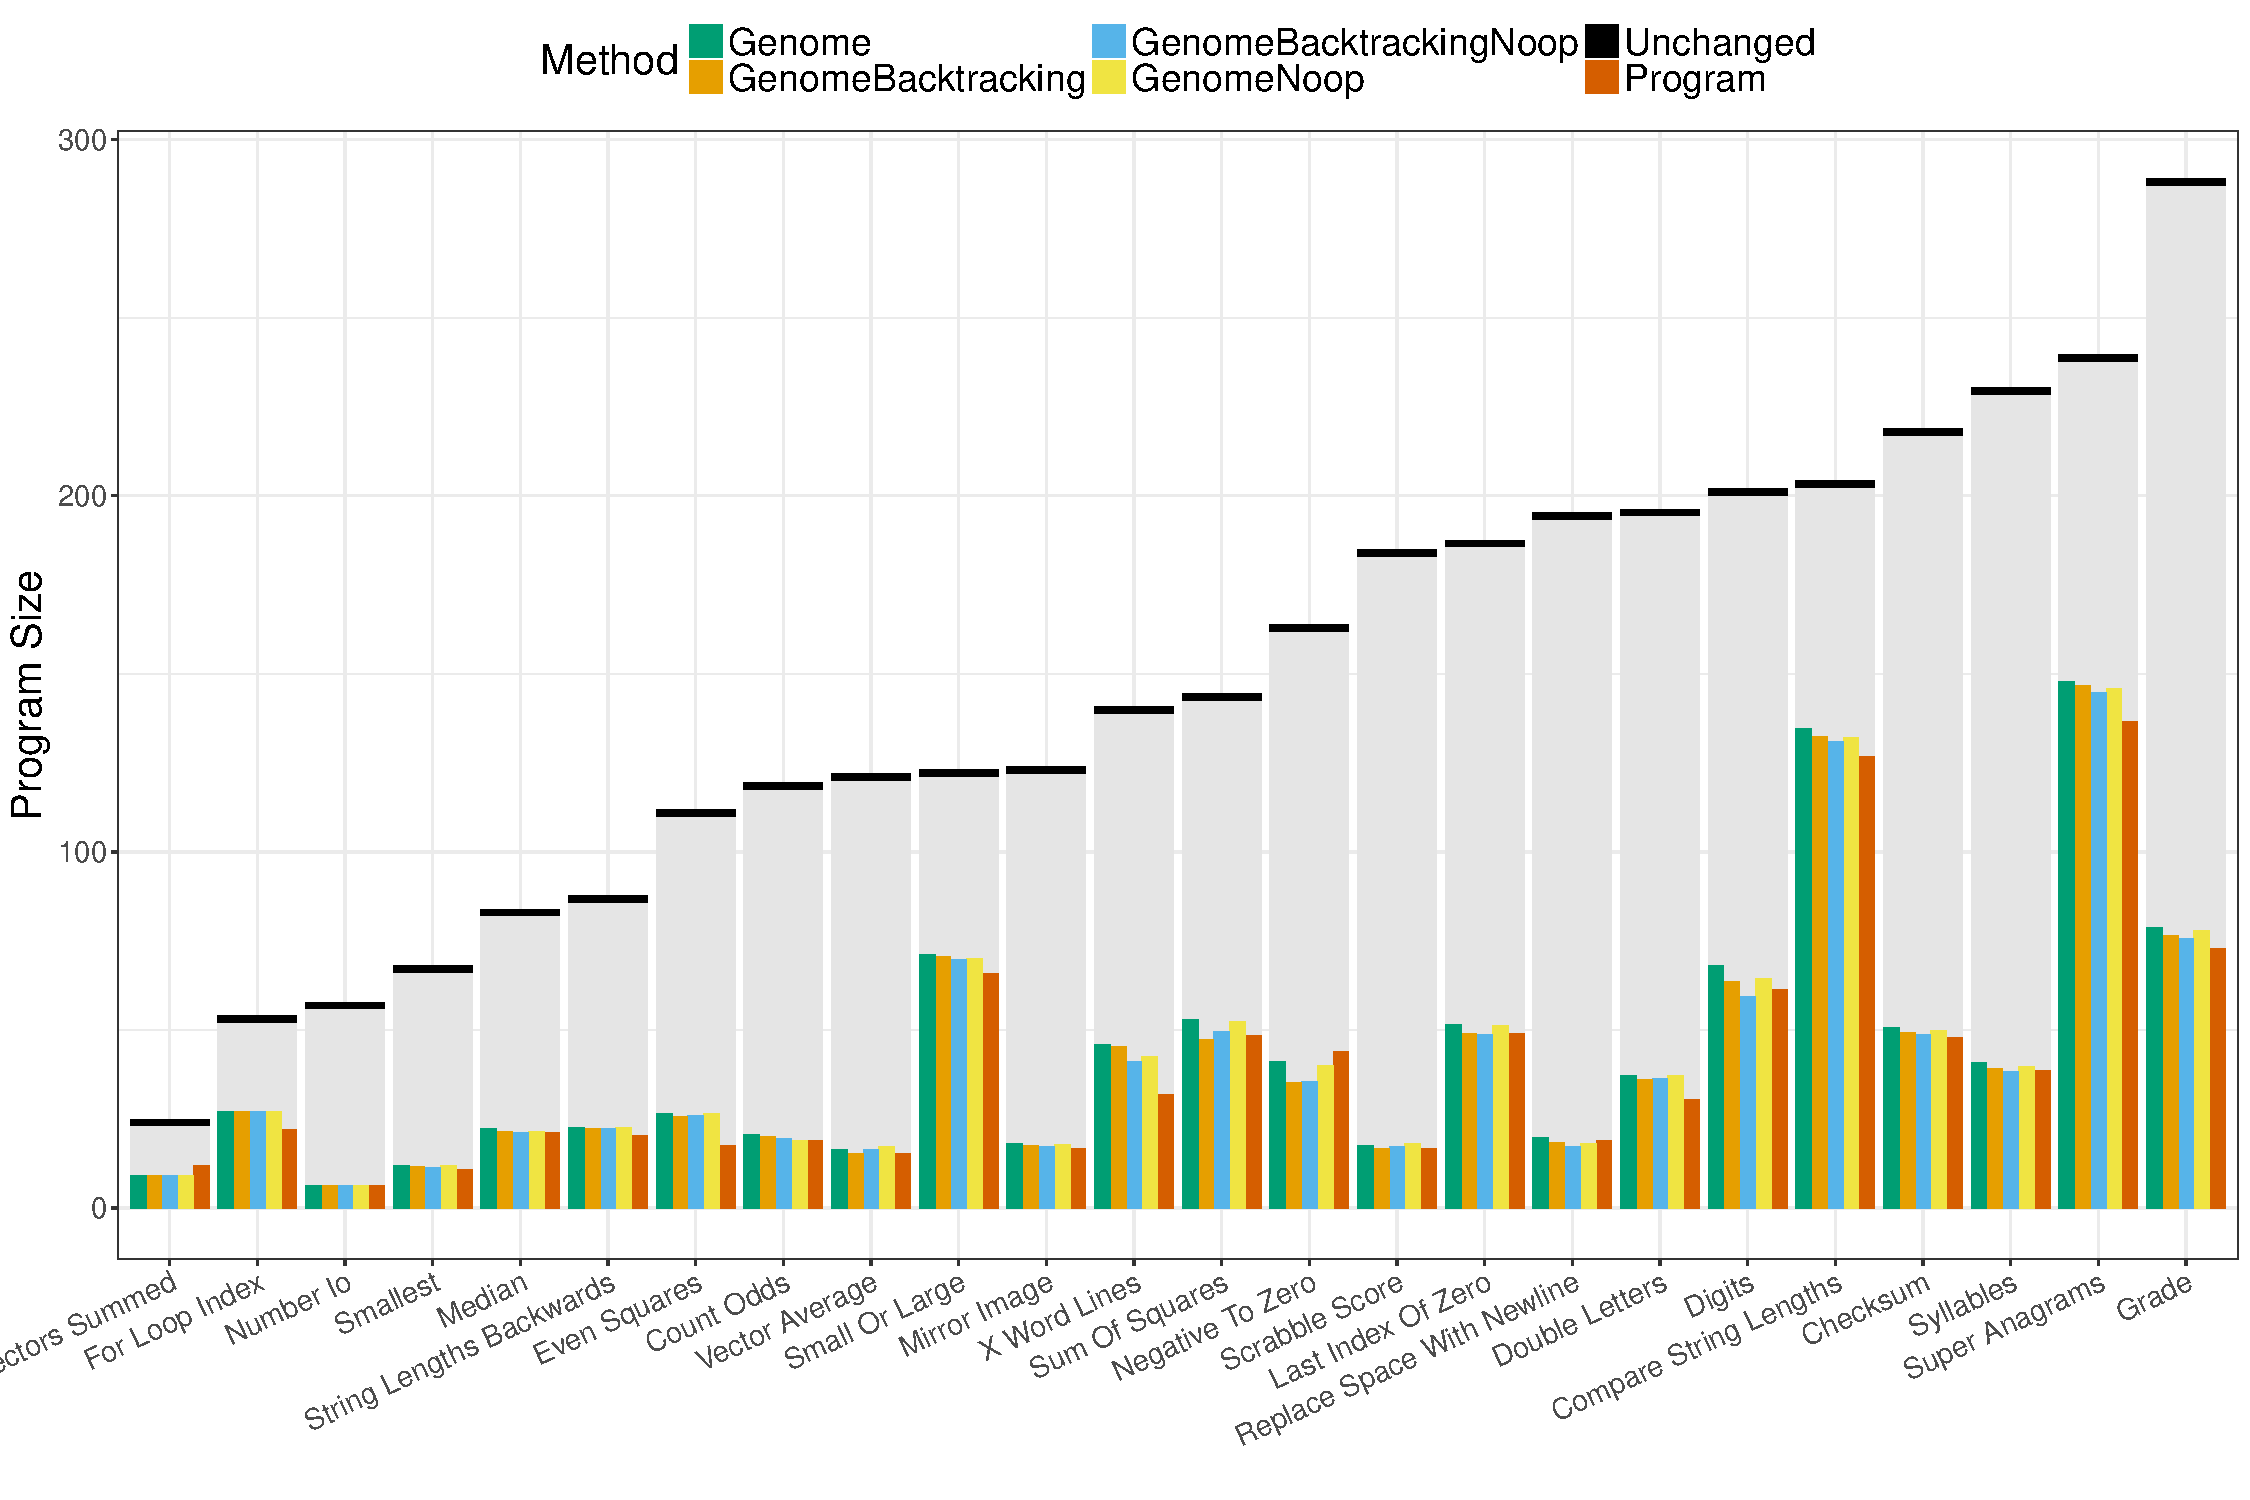
\includegraphics[width=\linewidth]{Illustrations/Problem_by_Size_bar_SLIDE}
\end{center}

\note{
	\begin{itemize}
		\item \emph{Explain the graph!}
		\item Reductions for all problems, most major
		\item A few see less dramatic reductions
		\begin{itemize}
			\item Small Or Large (33 sols)
			\item Compare String Lengths (60 sols)
			\item Super Anagrams (14 sols)
			\item All of these have low levels of generalizations; right-most three on previous graph
		\end{itemize}
		\item \emph{Doesn't seem to matter which simplification is used!}
	\end{itemize}
}

\end{frame}

\subsection{Improved generalization}

\begin{frame}{(Generally) improved generalization}

\begin{center}
	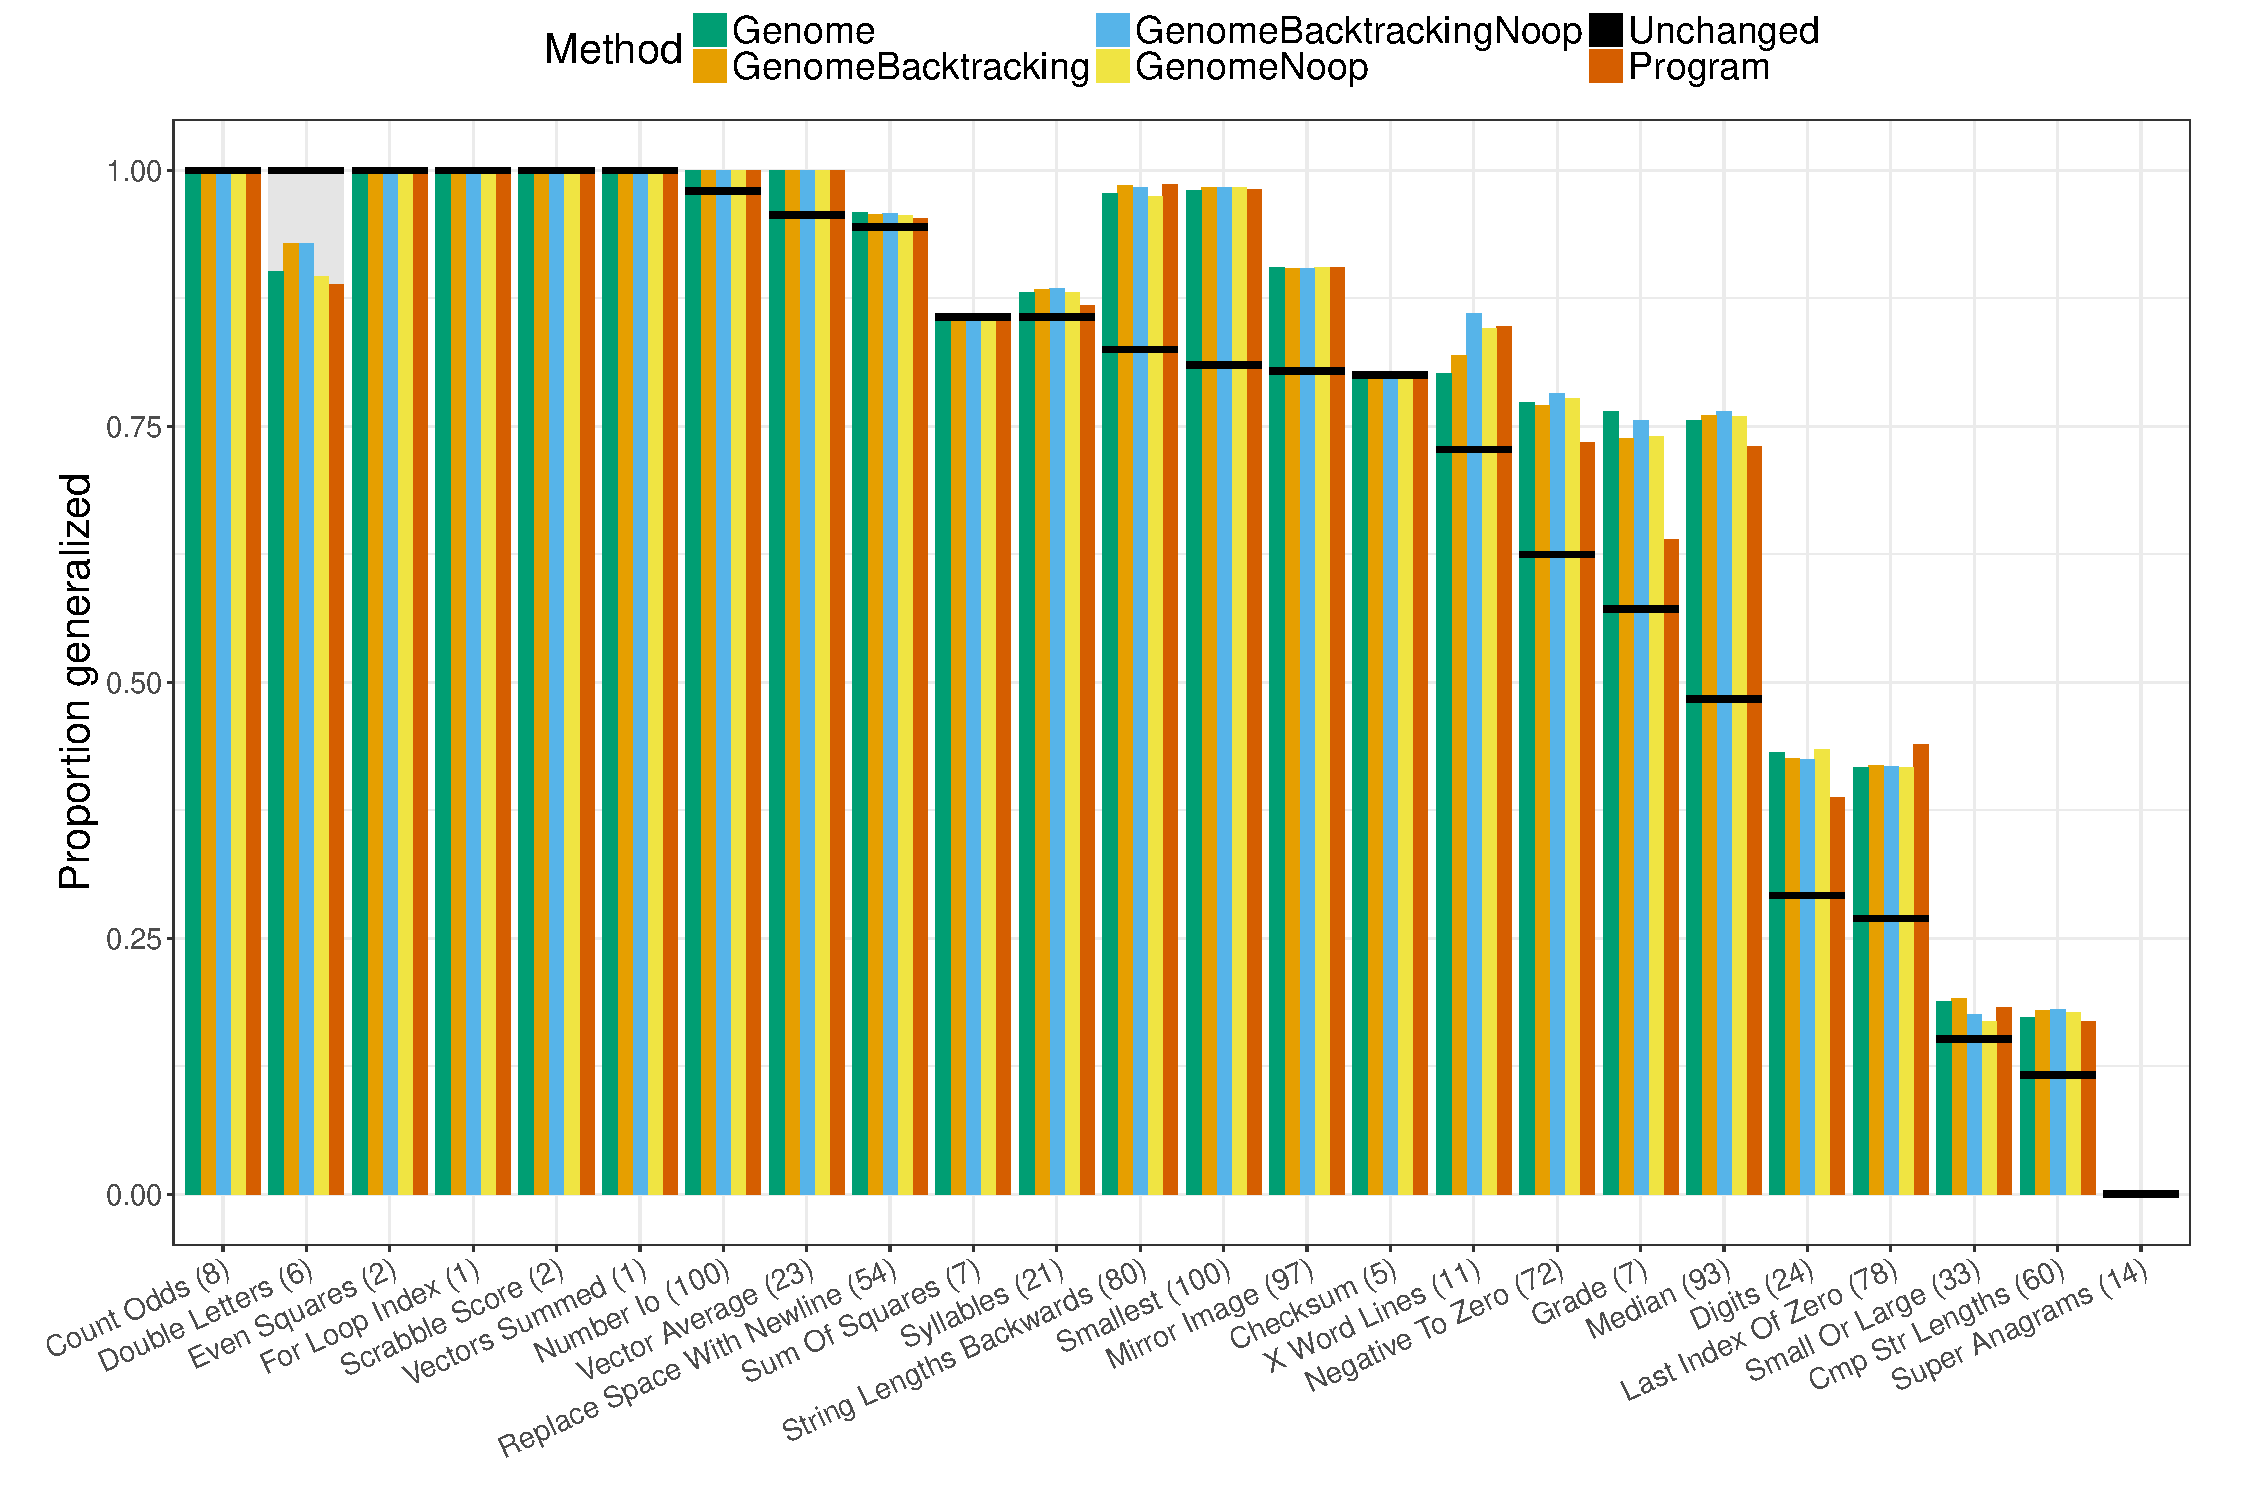
\includegraphics[width=0.95\linewidth]{Illustrations/Problem_by_PcntGen_bar_no_legend_SLIDE-3}
\end{center}

\note{
	\begin{itemize}
		\item \emph{Explain the graph!}
		\item Only one problem Double Letters sees a \emph{drop} in generalization
		\begin{itemize}
			\item Only 6 solutions, 5 of which generalize nicely after simplification; 1 didn't
		\end{itemize}
		\item 5 worst generalizers were among largest after simplification
		\begin{itemize}
			\item Simplification struggled to make them smaller, and often broke generalization.'
			\item Hypothesis: Sol'ns composed of ad hoc components that made them hard to simplify, and broke generalization, i.e., ``memorizing test cases''.
		\end{itemize}
		\item \emph{Again, doesn't matter much which simplification is used!}
	\end{itemize}
}

\end{frame}

\subsection{Discussion}

\begin{frame}{Most simplification methods about the same}

As the earlier graphs showed, no big differences in impact across different simplification methods

~

\begin{itemize}
	\item Shrinkage is statistically significant for all but \textbf{Genome}
	\item Generalization improvement versus unsimplified programs is statistically significant for all methods
\end{itemize}

\note{Using pairwise Freidman rank test (I think)}

\end{frame}

\begin{frame}{Short programs far more likely to generalize}
\begin{center}
	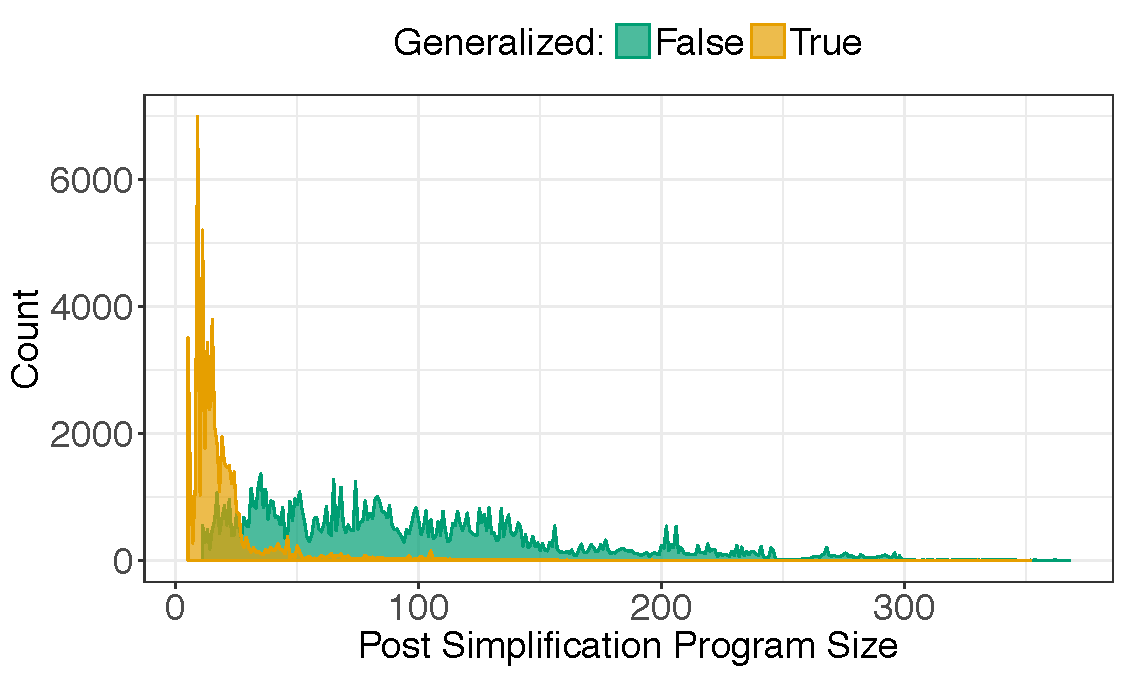
\includegraphics[width=0.9\linewidth]{Illustrations/Size_Density_final}
\end{center}

\end{frame}

\section{Conclusion}

\subsection*{Little dogs are cute}

\begin{frame}{Big wins all around! (generally)}

All methods led to substantial simplification on all problems
\begin{itemize}
	\item Typically cut program size by more than 50\%
\end{itemize}

~

All methods improved generalization on most problems
\begin{itemize}
	\item 65\% of programs generalized before simplification
	\item 76\% generalized after simplification
	\item Only hurt on one problem
	\item No change on a few
\end{itemize}

~

Do the \emph{results} generalize?
\begin{itemize}
	\item These results are fairly Push dependent
	\item Not obvious, e.g., how to directly map these ideas to trees
	\item Should be tried on, e.g., Linear GP, GE, Cartesian GP, etc.
\end{itemize}


\end{frame}

\begin{frame}{Thanks!}
\begin{columns}
\begin{column}{0.6\textwidth}
	\center \Large
	Thank you for your time \& attention! \\ \medskip
	
\includegraphics[width=.1\textwidth]{Illustrations/smile.png} \\ \medskip
	\normalsize
	~
	Special thanks to Bill Tozier, and the folks at the Computational Intelligence Lab at Hampshire College.
	
	~
	
	This material is based upon work supported by the National Science Foundation under 
	Grants No. 1129139 and 1331283.
\end{column}

\begin{column}{0.4\textwidth}
		\begin{center}
			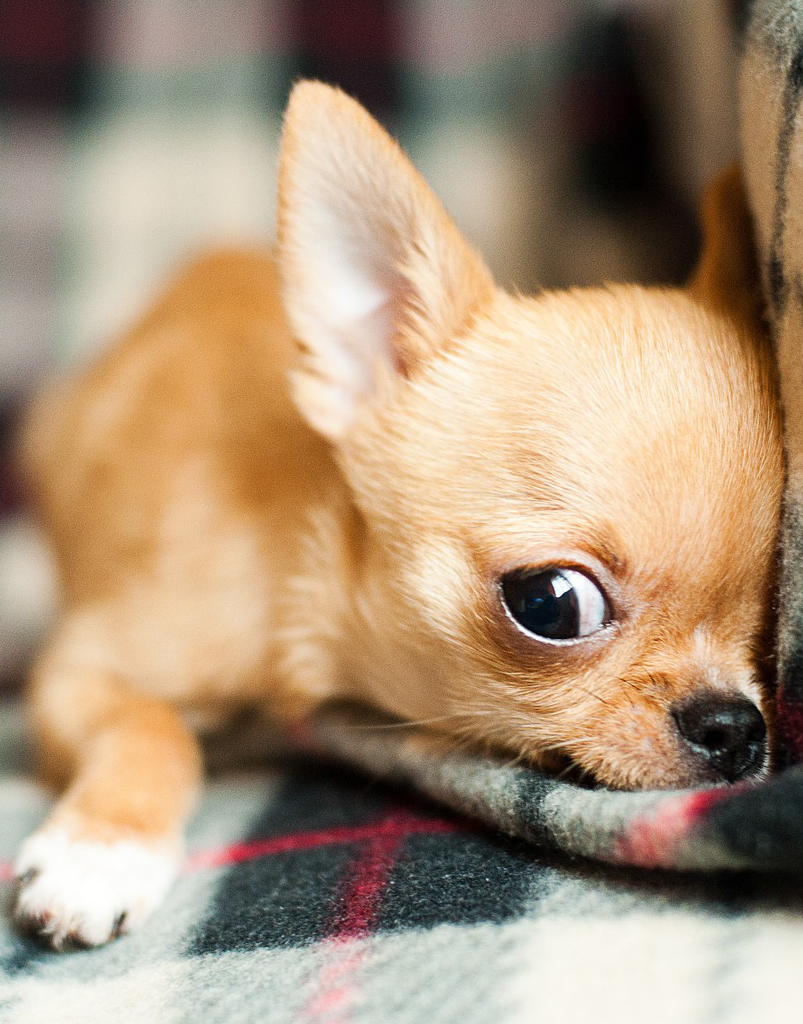
\includegraphics[height=0.7\textheight]{Illustrations/chihuahua-smaller} \\
			\tiny \url{https://pixabay.com/p-820086/}
		\end{center} 
	\end{column}
\end{columns}

\end{frame}

%~~~~~~~~~~References~~~~~~~~~~~~~~~~~~~~~~~~~~~~~~~~~~~~~~~~~~~~~~~~~~~~~~~~~~~~~~~~~~~~~~~~~~~~~~~~~~~~~~~

\section*{References}

\begin{frame}[allowframebreaks]
\frametitle{References}
\bibliographystyle{abbrv}
\bibliography{simplification.bib}
\end{frame}

\end{document}

\begin{frame} 
	\frametitle{References} 
	
	\begin{thebibliography}{lskdjf}
	\small 
	\bibitem{Burlacu:2013:GECCOcomp:new}
B.~Burlacu, M.~Affenzeller, M.~	Kommenda, S.~Winkler, and G.~Kronberger.
\newblock Visualization of genetic lineages and inheritance
information in genetic programming.
\newblock In Christian Blum, \emph{et al}, editors, {\em GECCO '13}, pages 1351--1358, New York, NY, USA, 2013.
	
	\bibitem{hyper:2016}
	T.~Helmuth, N.~F.~McPhee, and L.~Spector.
\newblock The Impact of Hyperselection on Lexicase Selection.
\newblock {\em GECCO '16}, Denver, CO, USA 2016.
  
	\bibitem{vis:2016}
	N.~F.~McPhee, M.~Casale, M.~Finzel, T.~Helmuth, and L.~Spector.
\newblock Visualizing genetic programming ancestries using graph databases.
\newblock {\em GECCO '16}, Denver, CO, USA 2016.
	
	\bibitem{gptp:2016}
	N.~F.~McPhee, M.~Finzel, M.~Casale, T.~Helmuth, and L.~Spector.
\newblock A detailed analysis of a PushGP run.
\newblock (Forthcoming) {\em GPTP '16}, Ann Arbor, MI, USA 2016.
	

  
  	\end{thebibliography}
	
\end{frame} 

